% !TeX root = ../../Book3.tex
% 纲要标题：## 第1章　黎曼度量与 Levi-Civita 联络
% 纲要位置：几何学计划纲要.md，第 2124 行。
% 正文状态：初稿；尚未正式审核。

% 纲要内容开始
% 
% > 本章目标与证明范围：从长度和度量相容性导出唯一无挠联络。公式必须能在坐标标架、正交标架和具体度量中互相核验；不把法坐标提前到指数映射之前。
% 
% 纲要内容结束

\chapter{黎曼度量与 Levi-Civita 联络}
\label{g3:ch:01}
\BookChapterNumber{g3:ch:01}

\begin{chapterabstract}
	光滑结构允许求导，黎曼度量进一步规定切向量的长度和夹角。本章由局部正定矩阵构造整体度量，建立梯度、体积密度、散度及分部积分公式；再从度量相容和无挠两个要求导出 Koszul 公式，证明 Levi-Civita 联络的存在唯一性。坐标标架与正交标架给出同一联络的两种表达，第一结构方程把无挠条件写成微分形式等式。诱导度量、乘积、共形变换和翘曲积展示这些公式的计算方式，二维模型与常数缩放则确定本卷的曲率符号和尺度约定。
\end{chapterabstract}

\begin{learninggoals}
	\begin{itemize}
		\item 从局部度量矩阵计算长度、梯度、体积密度与散度，并说明换坐标时这些几何量为何保持不变。
		\item 从度量相容和无挠条件推导 Koszul 公式，逐项验证它定义联络所需的线性及乘积法则。
		\item 在坐标标架和正交标架之间转换联络系数，用第一结构方程核验计算。
		\item 计算诱导、共形和翘曲积度量的联络，比较常数缩放对长度、体积和曲率的影响。
	\end{itemize}
\end{learninggoals}

在平面中，同一条曲线可以用直角坐标表示，也可以用极坐标表示。若曲线写成 \((r(t),\theta(t))\)，其速度的长度平方是
\[
	\dot r(t)^2+r(t)^2\dot\theta(t)^2.
\]
角度变化相同，在较大的圆周上走过的弧长就较长。这里的系数 \(r^2\) 记录坐标方向的实际尺度；它并不表示平面本身发生了弯曲。推广到流形时，我们在每个切空间上指定内积，并要求其系数随位置光滑变化。这使长度的定义脱离某一次坐标选择，也使没有预先嵌入空间的流形能够讨论体积和梯度。

\begin{figure}[htbp]
	\centering
	% !TeX root = ../Book3.tex
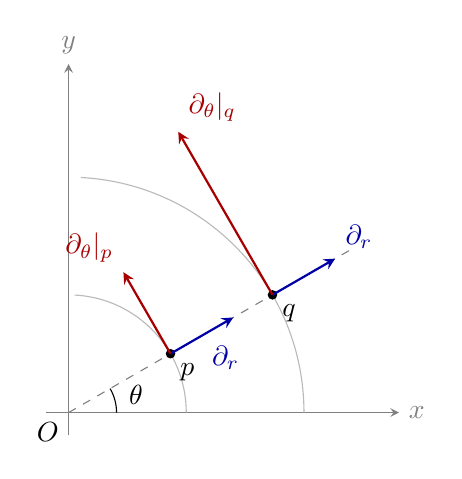
\begin{tikzpicture}[scale=1.15,>=stealth]
	\draw[->,gray] (-0.25,0)--(3.65,0) node[right]{\(x\)};
	\draw[->,gray] (0,-0.25)--(0,3.85) node[above]{\(y\)};
	\draw[gray!55] (0:1.3) arc[start angle=0,end angle=87,radius=1.3];
	\draw[gray!55] (0:2.6) arc[start angle=0,end angle=87,radius=2.6];
	\draw[dashed,gray] (0,0)--(30:3.6);
	\draw (0.53,0) arc[start angle=0,end angle=30,radius=0.53];
	\node at (15:0.77){\(\theta\)};
	\coordinate (P) at (30:1.3);
	\coordinate (Q) at (30:2.6);
	\fill (P) circle (1.5pt) node[below right]{\(p\)};
	\fill (Q) circle (1.5pt) node[below right]{\(q\)};
	\draw[->,thick,blue!65!black] (P)--++(30:0.8) node[midway,below right]{\(\partial_r\)};
	\draw[->,thick,blue!65!black] (Q)--++(30:0.8) node[above right]{\(\partial_r\)};
	\draw[->,thick,red!65!black] (P)--++(120:1.04) node[above left]{\(\partial_\theta|_p\)};
	\draw[->,thick,red!65!black] (Q)--++(120:2.08) node[above right]{\(\partial_\theta|_q\)};
	\node[below left] at (0,0){\(O\)};
\end{tikzpicture}

	\caption[极坐标方向的长度]{极坐标方向的长度。图中 \(q\) 的半径是 \(p\) 的两倍；用相同绘图比例表示向量时，两个径向坐标向量长度相同，角向坐标向量的长度则相差两倍。}
	\label{g3:fig:polar-coordinate-vectors}
\end{figure}

\cref{g3:fig:polar-coordinate-vectors}显示了度量如何记录坐标方向的尺度。有了长度，还需要比较邻近点的向量。在平面的极坐标标架中，径向和角向单位向量都随角度转动，所以只对向量的分量求导会漏掉标架本身的变化。联络把这部分变化计入导数。我们将要求这种导数满足内积的乘积法则，并使两个方向求导的反对称部分与向量场的括号一致。两个要求共同确定一个联络，其坐标表达和标架表达可以互相检验。

\ProseParagraphBreak

本章使用第一卷第11章的坐标图与切空间、第12章的张量和光滑单位分解，以及第14章的微分形式、密度积分和 Stokes 公式；每次实际调用时会恢复所需条件。\footnote{George Gabriel Stokes（1819--1903），生于爱尔兰的英国数学家、物理学家，研究流体力学与光学。}第一卷第15章学过的一般联络可帮助理解这些构造，本章仍给出切丛联络的定义和度量决定联络的证明。阅读本章无需先学第二卷的同调与同伦理论。度量给出曲线长度，长度的下确界如何成为距离、测地线如何产生法坐标，将在\chapref{g3:ch:02}展开。

\ProseParagraphBreak

以下光滑指 \(C^\infty\)，流形取有限维、Hausdorff、第二可数；除讨论边界积分时另作说明外，取实维数 \(n\ge1\) 且无边界。度量不要求可定向、紧或完备。坐标写为 \(x^1,\ldots,x^n\)，\(\partial_i\) 表示坐标向量场；同一单项式中重复的一个上指标和一个下指标表示从 \(1\) 到 \(n\) 求和。需要对照其他表述时，可参看 Petersen 第3版第1.1--1.2节和第1.4.2--1.4.4节的度量与标架、第2.2节和第2.4节的联络，以及第4.2.1节、第4.2.3节和第4.3.1节的球面与翘曲积模型\cite[第1.1--1.2节; 第1.4.2--1.4.4节; 第2.2节; 第2.4节; 第4.2.1节; 第4.2.3节; 第4.3.1节]{Petersen2016}。

% !TeX root = ../../Book3.tex
% 纲要标题：### 1.1 度量与几何量
% 纲要位置：几何学计划纲要.md，第 2128 行。
% 正文状态：初稿；尚未正式审核。

% 纲要内容开始
% 
% * 度量的存在及局部矩阵
% * 音乐同构、梯度和对偶度量
% * 体积密度、散度及分部积分
% * 坐标变化下的自然性
% 
% 纲要内容结束

\section{度量与几何量}
\label{g3:sec:0101}

一张坐标图能把曲线写成若干实函数，却没有规定哪个方向长、哪个方向短。即使在同一个平面上，\(\mathrm{d}x^2+\mathrm{d}y^2\) 与 \(4\,\mathrm{d}x^2+\mathrm{d}y^2\) 也给同一水平线段不同的长度。度量把这种测量规则放在每个切空间中，并要求它随点光滑变化。本节先说明度量怎样产生长度、梯度和体积，再由体积的变化定义散度；这些构造只需切丛、微分和积分，尚不需要比较不同点的向量。

\subsection{度量的存在及局部矩阵}
\label{g3:subsec:0101:01}

\begin{definition}
	\label{g3:def:riemannian-metric}
	设 \(M\) 是有限维、Hausdorff、第二可数的光滑流形。若光滑对称二阶协变张量场 \(g\) 在每个 \(p\in M\) 上给出正定双线性型 \(g_p\)，则称 \(g\) 为 \(M\) 上的\term[limanduliang]{黎曼度量}[Riemannian metric]，称 \((M,g)\) 为\term[limanliuxing]{黎曼流形}[Riemannian manifold]。向量的长度与非零向量之间的角度由
	\[
		|v|_g=\sqrt{g_p(v,v)},\qquad
		\cos\angle_g(v,w)=\frac{g_p(v,w)}{|v|_g|w|_g}
	\]
	确定。
\end{definition}

这个名称纪念 Riemann。\footnote{Riemann，德文全名 Georg Friedrich Bernhard Riemann（1826--1866），德国数学家，在复分析、几何及分析学中作出基础性贡献。}本章讨论 \(n\geq1\) 维光滑流形，通常无边界；涉及边界时另行说明。取局部坐标 \((x^1,\ldots,x^n)\)，写 \(\partial_i=\partial/\partial x^i\)。度量具有表达
\begin{equation}
	\label{g3:eq:metric-local-matrix}
	g=g_{ij}\,\mathrm{d}x^i\otimes\mathrm{d}x^j,\qquad
	g_{ij}=g(\partial_i,\partial_j).
\end{equation}
这里及后文对重复的一上一下指标求和；完整求和有时仍写出以便辨认。矩阵 \(G=(g_{ij})\) 对称正定，各分量光滑。反之，一组这样的局部矩阵，只要在交叠处遵守张量变换规律，就确定一个度量。\(\mathrm{d}x^i\mathrm{d}x^j\) 等常见的线元简写在本章均按相应对称双线性型理解；特别地，\(2g_{12}\,\mathrm{d}x^1\mathrm{d}x^2\) 包含两个对称交叉项。

\begin{proposition}
	\label{g3:prop:metric-existence}
	每个有限维、Hausdorff、第二可数的光滑流形都存在黎曼度量，允许流形有边界。若 \(g_0,g_1\) 是两个这样的度量，则 \((1-t)g_0+tg_1\) 在 \(0\leq t\leq1\) 时仍是黎曼度量。
\end{proposition}
\begin{proof}
	第一卷第12.3节的光滑单位分解定理（定理 12.3.5）说明：对任意坐标覆盖 \(\{U_\alpha\}\)，可取非负光滑函数 \(\rho_\alpha\)，使支集族局部有限、\(\operatorname{supp}\rho_\alpha\subset U_\alpha\)，且 \(\sum_\alpha\rho_\alpha=1\)。在 \(U_\alpha\) 上把坐标标架规定为正交单位标架，得到局部度量 \(h_\alpha\)。令
	\[
		g=\sum_\alpha\rho_\alpha h_\alpha,
	\]
	其中每项在 \(U_\alpha\) 外补零。支集包含关系使补零光滑，局部有限性使和在每点附近只有有限项。对非零 \(v\in\mathrm{T}_pM\)，各非零权重对应的 \(h_\alpha(v,v)\) 都为正，又至少有一个权重为正，故 \(g_p(v,v)>0\)。这正是第一卷丛度量构造在切丛上的应用。最后，两个正数的非负凸组合仍正，直接给出度量族的正定性。
\end{proof}

存在性依靠正定型的凸性，并没有给流形指定一个首选度量。度量一旦选定，曲线的长度便有确定含义。

\begin{definition}
	\label{g3:def:riemannian-length}
	设 \((M,g)\) 为黎曼流形，\(\gamma:[a,b]\to M\) 是分片 \(C^1\) 曲线。其\term[quxianchangdu]{长度}[length]定义为
	\[
		L_g(\gamma)=\int_a^b|\dot\gamma(t)|_g\,\mathrm{d}t
		=\int_a^b\sqrt{g_{ij}(\gamma(t))\dot x^i(t)\dot x^j(t)}\,\mathrm{d}t,
	\]
	右侧坐标表达在曲线的各个坐标片上分别计算并相加。
\end{definition}

被积量是切向量的内在长度，因而换坐标不改变结果。若 \(t=\phi(s)\) 是区间之间的 \(C^1\) 微分同胚，则链式法则给出 \(|(\gamma\circ\phi)'(s)|_g=|\phi'(s)|\,|\dot\gamma(\phi(s))|_g\)，换元后得到长度不变；递增与递减参数均可。正定性保证非零速度的长度为正。用所有连接两点的曲线长度取下确界会得到内在距离，其正定性与距离拓扑将在\chapref{g3:ch:02}证明。

\begin{proposition}
	\label{g3:prop:metric-coordinate-bounds}
	设 \(g\) 为光滑流形上的黎曼度量，\(K\) 是包含于一张坐标图 \(U\) 的非空紧集。存在常数 \(0<c\leq C<\infty\)，使对 \(p\in K\) 和 \(v=v^i\partial_i\in\mathrm{T}_pM\)，有
	\[
		c\sum_i(v^i)^2\leq g_p(v,v)\leq C\sum_i(v^i)^2.
	\]
\end{proposition}
\begin{proof}
	函数 \((p,a)\mapsto g_{ij}(p)a^ia^j\) 在紧集 \(K\times S^{n-1}\) 上连续且处处为正，故取得正的最小值 \(c\) 和有限最大值 \(C\)。对非零坐标向量先除以其 Euclid 长度，再利用二次齐次性；零向量时两式均成立。\footnote{Euclid（\OriginalName{Εὐκλείδης}，拉丁转写 Eukleidēs，约公元前300年活动，确切生卒年不详），古希腊数学家，活动于 Alexandria，以《几何原本》对几何与数论的系统论述著称。}
\end{proof}

这个估计把几何长度与坐标长度联系起来：曲线留在 \(K\) 时，两种长度分别相差至多因子 \(\sqrt c\) 与 \(\sqrt C\)。紧性使常数能够统一选择；在整个非紧坐标域上，未必存在同一对常数。例如 \(\mathbb R\) 上的 \(g=e^{2x}\mathrm{d}x^2\) 处处正定，但相对于 \(\mathrm{d}x^2\) 既没有全局正下界，也没有全局有限上界。

\subsection{音乐同构、梯度和对偶度量}
\label{g3:subsec:0101:02}

微分 \(\mathrm{d}f_p\) 接受方向并返回函数的变化率，是协变向量；描述“增长最快的方向”却需要一个向量。度量通过内积配对把这两类对象联系起来。

\begin{definition}
	\label{g3:def:musical-isomorphisms}
	黎曼流形 \((M,g)\) 的\term[yinyuetonggou]{音乐同构}[musical isomorphisms]是互逆的光滑丛同构
	\[
		\flat_g:\mathrm{T}M\longrightarrow\mathrm{T}^*M,
		\quad v^{\flat_g}=g(v,\mathord\cdot),
		\qquad
		\sharp_g:\mathrm{T}^*M\longrightarrow\mathrm{T}M.
	\]
	\(\sharp_g\) 由 \(g(\alpha^{\sharp_g},v)=\alpha(v)\) 刻画。度量明确时省略符号中的下标 \(g\)。
\end{definition}

正定性使 \(v\mapsto g(v,\mathord\cdot)\) 单射，有限维且两边维数相同，所以它可逆。记 \((g^{ij})=G^{-1}\)，则
\begin{equation}
	\label{g3:eq:musical-coordinates}
	(v^\flat)_i=g_{ij}v^j,\qquad
	(\alpha^\sharp)^i=g^{ij}\alpha_j.
\end{equation}
逆矩阵可由余子式除以 \(\det G>0\) 表示，所以逆映射也光滑。名称中的两个符号分别来自降号与升号，恰好对应把分量的指标降低和升高；它们依赖 \(g\)，并非切空间与余切空间原有的识别。

\begin{definition}
	\label{g3:def:dual-metric-gradient}
	黎曼流形 \((M,g)\) 的\term[duiouduliang]{对偶度量}[dual metric]是余切丛上的内积
	\[
		g^{-1}(\alpha,\beta)=g(\alpha^\sharp,\beta^\sharp)
		=g^{ij}\alpha_i\beta_j.
	\]
	对光滑实函数 \(f\)，其\term[tidu]{梯度}[gradient]为 \(\operatorname{grad}_g f=(\mathrm{d}f)^\sharp\)，即满足
	\begin{equation}
		\label{g3:eq:gradient-definition}
		g(\operatorname{grad}_g f,X)=Xf,\qquad
		\operatorname{grad}_g f=g^{ij}(\partial_jf)\partial_i
	\end{equation}
	的唯一光滑向量场。
\end{definition}

\symidx{\(\flat_g,\sharp_g\)}
\symidx{\(\operatorname{grad}_g f\)}

在 \(\mathrm{d}f_p\ne0\) 处，对所有单位向量 \(v\) 有
\[
	\mathrm{d}f_p(v)=g_p(\operatorname{grad}_g f,v)
	\leq|\operatorname{grad}_g f|_g,
\]
等号恰在 \(v=\operatorname{grad}_g f/|\operatorname{grad}_g f|_g\) 时成立。这来自内积不等式及其等号条件，也说明“最快”是以 \(g\) 的单位长度为尺度。若 \(M\) 无边界，且 \(\mathrm{d}f\) 在非空水平集 \(S=f^{-1}(c)\) 上处处非零，则第一卷第11.4节的正则水平集定理（定理 11.4.4）给出 \(\mathrm{T}_pS=\ker\mathrm{d}f_p\)，故梯度与水平集正交；在临界点，梯度为零，不再给出一个单位法向。

\begin{example}
	\label{g3:exm:gradient-metric-dependence}
	在 \(\mathbb R^2\) 上取 \(g=4\,\mathrm{d}x^2+\mathrm{d}y^2\) 与 \(f=x+y\)。则
	\[
		\mathrm{d}f=\mathrm{d}x+\mathrm{d}y,\qquad
		\operatorname{grad}_g f=\tfrac14\partial_x+\partial_y,
		\qquad |\mathrm{d}f|_{g^{-1}}^2=\tfrac54.
	\]
	水平线 \(x+y=c\) 的切向量 \(\partial_x-\partial_y\) 与这个梯度的 \(g\) 配对为 \(4\cdot\tfrac14-1=0\)。若换成 Euclid 度量，梯度变为 \(\partial_x+\partial_y\)，而 \(\mathrm{d}f\) 本身不变。逆矩阵出现在梯度公式中，正是为了补偿各方向长度尺度的不同。
\end{example}

同一个度量还在各阶张量丛上给出内积。例如对二阶协变张量 \(A\)，有 \(|A|_g^2=g^{ik}g^{j\ell}A_{ij}A_{k\ell}\)；对微分 \(k\) 形式，若写成 \(\alpha=\frac1{k!}\alpha_{i_1\cdots i_k}\mathrm{d}x^{i_1}\wedge\cdots\wedge\mathrm{d}x^{i_k}\)，则
\[
	|\alpha|_g^2=\frac1{k!}
	g^{i_1j_1}\cdots g^{i_kj_k}
	\alpha_{i_1\cdots i_k}\alpha_{j_1\cdots j_k}.
\]
因子 \(1/k!\) 消去同一有序指标组的排列重复，使正交余标架中递增指标的楔积成为正交单位基。

\subsection{体积密度、散度及分部积分}
\label{g3:subsec:0101:03}

切空间中的内积还确定平行多面体的体积。对切向量组 \((v_1,\ldots,v_n)\)，其体积为内积矩阵 \((g(v_i,v_j))\) 行列式的非负平方根。换基矩阵若为 \(A\)，内积矩阵变为 \(A^{\mathsf T}GA\)，体积就乘以 \(|\det A|\)。这提示应使用绝对行列式变换的密度，而不必先选择定向。

\begin{definition}
	\label{g3:def:metric-volume-density}
	\(n\) 维黎曼流形 \((M,g)\) 的\term[tijimidu]{体积密度}[volume density]记为 \(\mu_g\)，在坐标中写为
	\begin{equation}
		\label{g3:eq:volume-density}
		\mu_g=\sqrt{\det G}\,|\mathrm{d}x^1\cdots\mathrm{d}x^n|.
	\end{equation}
	若另外给定定向，则在正向坐标中
	\[
		\operatorname{vol}_g=\sqrt{\det G}\,\mathrm{d}x^1\wedge\cdots\wedge\mathrm{d}x^n
	\]
	定义相应的\term[tijixingshi]{体积形式}[volume form]。
\end{definition}

\symidx{\(\mu_g\)}

密度符号中的竖线表示换坐标时取绝对行列式，不是对微分符号求绝对值。第一卷第14.3节的积分良定义定理（定理 14.3.4）已证明：将紧支光滑密度用单位分解拆到坐标片后，按通常多元积分求和，结果与坐标和分解无关。因此 \(\int_M f\mu_g\) 对紧支光滑 \(f\) 有定义，不要求 \(M\) 可定向。一般非负可测函数的体积积分可由这一光滑正密度所给的局部测度定义；本章的分部积分只用紧支光滑情形。定向反转会改变 \(\operatorname{vol}_g\) 的符号，却不改变 \(\mu_g\)。

\ProseParagraphBreak

散度测量向量场的流对体积的一阶改变。设 \(X\) 是无边界流形上的光滑向量场。第一卷第13.1节的最大局部流定理（定理 13.1.7）给出随 \((t,p)\) 光滑变化的局部微分同胚 \(\Phi_t\)，满足 \(\Phi_0=\operatorname{id}\) 与 \(\partial_t\Phi_t=X\circ\Phi_t\)。密度的\term[liedaoshu]{Lie 导数}[Lie derivative]定义为 \(\mathcal L_X\mu_g=\left.\frac{\mathrm{d}}{\mathrm{d}t}\right|_{t=0}\Phi_t^*\mu_g\)。\footnote{Lie，Marius Sophus Lie（1842--1899），挪威数学家，创立连续变换群理论，并研究其与微分方程的联系。}这里只需在每一点附近对足够小的 \(t\) 定义流，无需假设流对所有时间存在。由于 \(\mu_g\) 处处正，存在唯一光滑函数满足
\begin{equation}
	\label{g3:eq:divergence-definition}
	\mathcal L_X\mu_g=(\operatorname{div}_gX)\mu_g.
\end{equation}
这个函数称为 \(X\) 的\term[sandu]{散度}[divergence]。

\begin{proposition}
	\label{g3:prop:divergence-coordinate}
	在无边界黎曼流形 \((M,g)\) 的任一坐标图中，对光滑向量场 \(X=X^i\partial_i\)，有
	\begin{equation}
		\label{g3:eq:divergence-coordinate}
		\operatorname{div}_gX
		=\frac1{\sqrt{\det G}}\partial_i\bigl(\sqrt{\det G}\,X^i\bigr).
	\end{equation}
	因此，对光滑实函数 \(f\)，有
	\begin{equation}
		\label{g3:eq:divergence-product}
		\operatorname{div}_g(fX)=\mathrm{d}f(X)+f\operatorname{div}_gX.
	\end{equation}
	公式也唯一地延伸到带边界流形上光滑至边界的向量场。
\end{proposition}
\begin{proof}
	记 \(m=\sqrt{\det G}\)。局部流拉回密度的系数为 \(m(\Phi_t(x))|\det\mathrm{D}\Phi_t(x)|\)。在 \(t=0\) 时，\(\Phi_0=\operatorname{id}\)，且 \(\left.\partial_t\Phi_t\right|_0=X\)。行列式在单位矩阵处的一阶项是迹，故
	\[
		\left.\frac{\mathrm{d}}{\mathrm{d}t}\right|_0
		\bigl(m(\Phi_t(x))|\det\mathrm{D}\Phi_t(x)|\bigr)
		=X^i\partial_i m+m\partial_iX^i=\partial_i(mX^i).
	\]
	除以 \(m>0\) 即得坐标公式；对 \(fX\) 展开偏导数得到乘积公式。若流形有边界，坐标系数在半空间边界处仍光滑；不同边界图中的表达在稠密的内部相同，连续性使它们在边界也相同。这样定义边界处的散度，无须要求 \(X\) 的双侧流保留流形。
\end{proof}

在定向坐标片中，直接将 \(\iota_X\operatorname{vol}_g\) 写成缺少一个坐标微分的各项可得
\begin{equation}
	\label{g3:eq:divergence-exterior}
	\mathrm{d}(\iota_X\operatorname{vol}_g)
	=(\operatorname{div}_gX)\operatorname{vol}_g.
\end{equation}
这里 \(\iota_X\) 将 \(X\) 插入形式的第一个位置；各项的排列符号恰好使外微分的系数成为 \(\partial_i(mX^i)\)。由此可以把散度积分转成边界通量。

\ProseParagraphBreak

若 \(M\) 有光滑边界，限制 \(g\) 到 \(\mathrm{T}\partial M\) 就给出边界度量，记它的体积密度为 \(\mu_{\partial g}\)。在边界坐标中取定义函数 \(r\)，使 \(M\) 对应 \(r\geq0\)、边界对应 \(r=0\)，且边界上 \(\mathrm{d}r\ne0\)。于是 \(\nu=-\operatorname{grad}_g r/|\operatorname{grad}_g r|_g\) 是外单位法向。它由正交、单位长度和向外这三个条件唯一确定，所以不同边界图中的选择相容。

\begin{theorem}[散度定理]
	\label{g3:thm:divergence-theorem}
	设 \((M^n,g)\) 为有限维、Hausdorff、第二可数的光滑黎曼流形，\(n\geq1\)，允许有光滑边界，无须可定向。若 \(X\) 是光滑至边界的紧支向量场，\(\nu\) 是边界的外单位法向，\(\mu_{\partial g}\) 是边界诱导度量的体积密度，则
	\begin{equation}
		\label{g3:eq:divergence-theorem}
		\int_M\operatorname{div}_gX\,\mu_g
		=\int_{\partial M}g(X,\nu)\,\mu_{\partial g}.
	\end{equation}
	无边界时右侧为零；\(n=1\) 时边界积分按各端点的计数密度求和。
\end{theorem}
\begin{proof}
	先假设 \(X\) 的支集位于一张坐标片 \(U\) 内并紧含于该片。给 \(U\) 任选定向，对紧支形式 \(\iota_X\operatorname{vol}_g\) 使用第一卷第14.4节的 Stokes 定理（定理 14.4.3）：外微分的积分等于在外法向优先定向下的边界积分。由\eqref{g3:eq:divergence-exterior}，左边就是散度乘以正体积密度的积分。

	当 \(n\geq2\) 时，在边界点取正交单位基 \((\nu,e_1,\ldots,e_{n-1})\)，使它符合 \(U\) 的定向。把 \(X\) 分成法向部分 \(g(X,\nu)\nu\) 和切向部分，切向部分与其余 \(n-1\) 个切向量线性相关，因而在顶次形式中贡献为零。故
	\[
		(\iota_X\operatorname{vol}_g)(e_1,\ldots,e_{n-1})=g(X,\nu).
	\]
	所以边界项正是 \(g(X,\nu)\mu_{\partial g}\) 的积分。\(n=1\) 时，在正向单位切向量为 \(e\) 的记号下，若 \(\nu=\varepsilon e\)，边界点的诱导定向符号就是 \(\varepsilon\)；其贡献为 \(\varepsilon\operatorname{vol}_g(X)=g(X,\nu)\)，结论相同。反转所选定向会同时反转体积形式与边界定向，两个密度积分都不变，所得局部公式不依赖这次选择。

	一般情形取从属于坐标覆盖的光滑单位分解 \(\{\rho_\alpha\}\)。紧支性及局部有限性保证只有有限个 \(\rho_\alpha X\) 非零，且各项支集紧含于相应坐标片。逐项应用局部公式并相加。乘积公式给出
	\[
		\sum_\alpha\operatorname{div}_g(\rho_\alpha X)
		=\Bigl(\sum_\alpha\rho_\alpha\Bigr)\operatorname{div}_gX
		+X\Bigl(\sum_\alpha\rho_\alpha\Bigr)
		=\operatorname{div}_gX,
	\]
	边界通量的和也等于 \(g(X,\nu)\)。这证明全局公式，包括不可定向情形。
\end{proof}

把定理应用于 \(fX\)，得到分部积分的基本形式。若 \(f\) 光滑、\(X\) 光滑，且其中至少一个紧支，则
\begin{equation}
	\label{g3:eq:integration-by-parts}
	\int_M f\operatorname{div}_gX\,\mu_g
	=-\int_M g(\operatorname{grad}_g f,X)\,\mu_g
	+\int_{\partial M}f g(X,\nu)\,\mu_{\partial g}.
\end{equation}
在带边界情形，所有数据都要求光滑至边界。无边界、\(f\) 在边界为零，或 \(X\) 沿边界切向时，边界项消失。非紧流形上的支集条件则控制无穷远的通量，不能从公式中直接删除。

\begin{definition}
	\label{g3:def:laplace-beltrami}
	对黎曼流形上的光滑实函数 \(f\)，采用\term[laplacebeltramisuanzi]{Laplace--Beltrami 算子}[Laplace--Beltrami operator]的非负号约定
	\begin{equation}
		\label{g3:eq:laplace-beltrami}
		\Delta_g f\coloneqq-\operatorname{div}_g(\operatorname{grad}_g f)
		=-\frac1{\sqrt{\det G}}
		\partial_i\bigl(\sqrt{\det G}\,g^{ij}\partial_jf\bigr).
	\end{equation}
\end{definition}

\symidx{\(\operatorname{div}_g X\)}
\symidx{\(\Delta_g\)}

这个名称沿用 Laplace 和 Beltrami 的姓氏。\footnote{Laplace，法文全名 Pierre-Simon Laplace（1749--1827），法国数学家和天文学家，研究概率、势函数与天体力学。Beltrami，意大利文名 Eugenio Beltrami（1835--1900），意大利数学家，研究微分几何、非 Euclid 几何模型及微分算子。}具体说，无边界时，对 \(u,v\in C_c^\infty(M)\)，分部积分给出
\begin{equation}
	\label{g3:eq:laplace-energy}
	\int_M u\Delta_gv\,\mu_g
	=\int_M g(\operatorname{grad}_g u,\operatorname{grad}_g v)\,\mu_g
	=\int_M v\Delta_gu\,\mu_g.
\end{equation}
令 \(u=v\)，便有 \(\int_Mu\Delta_gu\,\mu_g\geq0\)。这说明本书的非负号约定指积分二次型非负，不是说每个非负函数的 \(\Delta_g\) 仍逐点非负。带边界时，对光滑至边界的紧支函数 \(u,v\)，相应公式为
\[
	\int_Mu\Delta_gv\,\mu_g
	=\int_M g(\operatorname{grad}_g u,\operatorname{grad}_g v)\,\mu_g
	-\int_{\partial M}u\partial_\nu v\,\mu_{\partial g},
\]
其中 \(\partial_\nu v=\mathrm{d}v(\nu)\)。例如两函数都在边界为零时，仍得到\eqref{g3:eq:laplace-energy}的对称关系。

\begin{example}
	\label{g3:exm:polar-metric-operators}
	在平面去掉原点后的一个角度坐标片上，Euclid 度量写为
	\[
		g=\mathrm{d}r^2+r^2\mathrm{d}\theta^2,\qquad
		\mu_g=r|\mathrm{d}r\,\mathrm{d}\theta|.
	\]
	因此
	\[
		\begin{aligned}
			\operatorname{grad}_g f
			&=f_r\partial_r+r^{-2}f_\theta\partial_\theta,\\
			\operatorname{div}_g X
			&=r^{-1}\partial_r(rX^r)+\partial_\theta X^\theta,\\
			\Delta_g f
			&=-f_{rr}-r^{-1}f_r-r^{-2}f_{\theta\theta}.
		\end{aligned}
	\]
	这里 \(X^\theta\) 是相对于 \(\partial_\theta\) 的系数；若改用单位向量 \(r^{-1}\partial_\theta\) 的系数，散度的角向项也必须相应改写。例如 \(X=\partial_r\) 满足 \(\operatorname{div}_gX=1/r\)：向外移动厚度相同的小扇环，其周长随半径增长。原点不属于这张坐标图，公式中的 \(1/r\) 不表示原平面的度量在原点有奇性。
\end{example}

\subsection{坐标变化下的自然性}
\label{g3:subsec:0101:04}

前面的公式都含矩阵逆、行列式和偏导数。它们能否给出同一个几何对象，取决于这些变化是否彼此抵消。先直接核对换坐标，再把结论表述为局部等距下的相容性。

\ProseParagraphBreak

在交叠坐标 \(x=x(y)\) 中，记 \(J^i{}_a=\partial x^i/\partial y^a\)。由 \(\partial/\partial y^a=J^i{}_a\partial_i\)，新矩阵满足
\begin{equation}
	\label{g3:eq:metric-coordinate-transformation}
	G_y=J^{\mathsf T}G_xJ,\qquad
	G_y^{-1}=J^{-1}G_x^{-1}(J^{\mathsf T})^{-1},\qquad
	\sqrt{\det G_y}=|\det J|\sqrt{\det G_x}.
\end{equation}
第一式是双线性型的换基，第二式保证升指标后得到向量的变换规律，第三式恰是密度的变换规律。因此 \(g^{-1}\)、梯度和 \(\mu_g\) 的局部表达在交叠处相容；散度由局部流定义，也与坐标选择无关。

\begin{definition}
	\label{g3:def:local-isometry}
	设 \((M,g)\)、\((N,h)\) 是黎曼流形。若光滑映射 \(F:M\to N\) 是局部微分同胚且 \(F^*h=g\)，即
	\[
		h_{F(p)}(\mathrm{d}F_pv,\mathrm{d}F_pw)=g_p(v,w),
	\]
	则称 \(F\) 为\term[jubudengju]{局部等距}[local isometry]。若它还是微分同胚，则称为\term[dengju]{等距}[isometry]。
\end{definition}

\begin{proposition}
	\label{g3:prop:metric-naturality}
	设 \(F:(M,g)\to(N,h)\) 是无边界黎曼流形间的局部等距，\(f\in C^\infty(N)\)。则
	\[
		F^*\mu_h=\mu_g,\qquad
		\mathrm{d}F\bigl(\operatorname{grad}_g(f\circ F)\bigr)
		=(\operatorname{grad}_h f)\circ F,
	\]
	且对任意分片 \(C^1\) 曲线 \(\gamma\)，有 \(L_h(F\circ\gamma)=L_g(\gamma)\)。若向量场 \(X\) 与 \(Y\) 满足 \(\mathrm{d}F(X)=Y\circ F\)，则
	\[
		\operatorname{div}_gX=(\operatorname{div}_hY)\circ F,
		\qquad \Delta_g(f\circ F)=(\Delta_h f)\circ F.
	\]
\end{proposition}
\begin{proof}
	密度等式由\eqref{g3:eq:metric-coordinate-transformation}的行列式关系得出，长度等式由 \(\mathrm{d}F\) 逐点保持速度的内积得出。对任意 \(v\in\mathrm{T}_pM\)，有
	\[
		\begin{aligned}
			h\bigl(\mathrm{d}F\operatorname{grad}_g(f\circ F),\mathrm{d}Fv\bigr)
			&=\mathrm{d}(f\circ F)(v)\\
			&=\mathrm{d}f(\mathrm{d}Fv)
			=h\bigl(\operatorname{grad}_h f,\mathrm{d}Fv\bigr).
		\end{aligned}
	\]
	因 \(\mathrm{d}F_p\) 满射且 \(h\) 非退化，得到梯度关系。

	最后把 \(F\) 限制在可逆的邻域中，在目标选择坐标 \(y\)，源上取 \(x=y\circ F\)。相关向量场在这两套对应坐标中的分量相同，\(G(x)=H(y)\) 也对应相同。因此\eqref{g3:eq:divergence-coordinate}在对应点给出同一实数，证明散度关系。将它用于刚得到的梯度关系，再带入 \(\Delta=-\operatorname{div}\operatorname{grad}\)，便得到最后一个等式。
\end{proof}

局部等距可以重复覆盖同一个区域。例如 \(\mathbb R\to S^1\)、\(t\mapsto(\cos t,\sin t)\)，对 \(\mathrm{d}t^2\) 与单位圆的诱导度量是局部等距，它保持每条参数曲线的长度，却不保持整个空间的总体积。积分换元还需整体条件：若 \(F\) 是等距、\(f\in C_c^\infty(N)\)，则第一卷定理 14.3.6 的密度换元给出 \(\int_M(f\circ F)\mu_g=\int_Nf\mu_h\)；若仅有局部等距，重叠覆盖的次数可能改变积分。矩阵变换、局部几何量和整体积分因而各自有清楚的适用范围。

% !TeX root = ../../Book3.tex
% 纲要标题：### 1.2 Levi-Civita 定理
% 纲要位置：几何学计划纲要.md，第 2135 行。
% 正文状态：未撰写；本文件目前是框架。

% 纲要内容开始
% 
% * 度量相容与无挠的独立要求
% * Koszul 公式的推导
% * 由公式构造联络并验证性质
% * 存在唯一性及 Christoffel 表达
% 
% 纲要内容结束

\section{Levi-Civita 定理}
\label{g3:sec:0102}

待撰写

\subsection{度量相容与无挠的独立要求}
\label{g3:subsec:0102:01}
待撰写

\subsection{Koszul 公式的推导}
\label{g3:subsec:0102:02}
待撰写

\subsection{由公式构造联络并验证性质}
\label{g3:subsec:0102:03}
待撰写

\subsection{存在唯一性及 Christoffel 表达}
\label{g3:subsec:0102:04}
待撰写
% 纲要条目排为编号小节标题，并进入目录与书签；说明段仍保留于纲要注释中。

% !TeX root = ../../Book3.tex
% 纲要标题：### 1.3 标架与结构方程
% 纲要位置：几何学计划纲要.md，第 2142 行。
% 正文状态：初稿；尚未正式审核。

% 纲要内容开始
% 
% * 正交标架和联络一形式
% * Cartan 第一结构方程
% * 曲率形式的预告与符号约定
% 
% 纲要内容结束

\section{标架与结构方程}
\label{g3:sec:0103}

坐标标架的优点是向量场两两交换，代价是度量矩阵往往随点变化。若在每点把基改成正交单位基，度量矩阵就恒为单位矩阵，但新的基向量场通常不再交换。联络一形式和结构方程把这两种变化一起记录下来，使度量的计算可以在适合几何形状的标架中进行。

\subsection{正交标架和联络一形式}
\label{g3:subsec:0103:01}

给定局部光滑标架 \((v_1,\ldots,v_n)\)，依次作正交化：
\[
	e_1=\frac{v_1}{|v_1|_g},\qquad
	w_j=v_j-\sum_{a<j}g(v_j,e_a)e_a,\qquad
	e_j=\frac{w_j}{|w_j|_g}.
\]
各 \(w_j\) 处处非零，因为原标架线性无关；平方范数为正的光滑函数，其平方根和倒数光滑。因此这给出光滑的\term[zhengjiaodanweibiaojia]{正交单位标架}[orthonormal frame]。局部存在这样的标架不要求流形可定向。

\begin{definition}\label{g3:def:connection-one-forms}
	设 \((M,g)\) 为光滑黎曼流形，\(\nabla\) 为其 Levi-Civita 联络。在开集 \(U\) 上取光滑行标架 \(e=(e_1,\ldots,e_n)\)，以
	\[
		\nabla_Xe_j=e_i\omega^i{}_j(X)
	\]
	定义\term[lianluoyixingshi]{联络一形式}[connection one-forms] \(\omega^i{}_j\)，并记矩阵 \(\omega=(\omega^i{}_j)\)。若 \(u\) 为分量列，则
	\begin{equation}\label{g3:eq:frame-connection}
		\nabla_X(eu)=e\bigl(X(u)+\omega(X)u\bigr),\qquad
		\nabla e=e\omega.
	\end{equation}
	对偶余标架写为列 \(\theta=(\theta^1,\ldots,\theta^n)^{\mathsf T}\)，满足 \(\theta^i(e_j)=\delta^i_j\)，故 \(X=e\theta(X)\)。
\end{definition}

上下指标的位置记录输入与输出：\(j\) 指被微分的标架向量，\(i\) 指结果的分量；求导方向留给一形式接受。在坐标标架中，\(\omega^k{}_j=\Gamma^k_{ij}\,\mathrm{d}x^i\)。这与第一卷第15章的行标架、列分量约定一致，该卷将一般丛的联络矩阵记作 \(A\)。

\begin{proposition}\label{g3:prop:frame-metric-and-change}
	设 \((M,g)\) 为光滑黎曼流形，\(\nabla\) 为与 \(g\) 相容的光滑联络。在局部标架 \(e\) 中记 \(G=(g(e_i,e_j))\)，联络矩阵为 \(\omega\)。则
	\[
		\mathrm{d}G=\omega^{\mathsf T}G+G\omega.
	\]
	特别地，在正交单位标架中，\(\omega^i{}_j=-\omega^j{}_i\)。若 \(e'=eQ\)，其中 \(Q:U\to\operatorname{O}(n)\) 为光滑正交矩阵函数，则
	\begin{equation}\label{g3:eq:orthonormal-frame-change}
		\omega'=Q^{-1}\omega Q+Q^{-1}\mathrm{d}Q,\qquad
		\theta'=Q^{-1}\theta.
	\end{equation}
\end{proposition}
\begin{proof}
	度量相容性给出
	\[
		\mathrm{d}\bigl(g(e_i,e_j)\bigr)
		=\omega^k{}_i g(e_k,e_j)+g(e_i,e_k)\omega^k{}_j,
	\]
	即所述矩阵等式。若 \(G=I\)，左侧为零，便得到斜对称性。换标架时，对 \(eQ\) 使用乘积规则：
	\[
		\nabla e'=e(\omega Q+\mathrm{d}Q)
		=e'Q^{-1}(\omega Q+\mathrm{d}Q).
	\]
	与 \(\nabla e'=e'\omega'\) 比较即得第一式。由 \(X=e\theta(X)=eQ\theta'(X)\) 得第二式。
\end{proof}

正交标架的度量系数虽为常数，联络系数仍可非零。若 \([e_i,e_j]=c^k{}_{ij}e_k\)，将三个标架向量代入 Koszul 公式，得到
\begin{equation}\label{g3:eq:orthonormal-koszul}
	2\omega^k{}_j(e_i)=c^k{}_{ij}-c^i{}_{jk}+c^j{}_{ki}.
\end{equation}
度量的变化现在由标架向量的括号表达。特别地，若正交单位标架的所有括号都为零，则此标架中的联络矩阵为零。

\subsection{Cartan 第一结构方程}
\label{g3:subsec:0103:02}

余标架 \(\theta\) 把实际切向量转为标架分量。它的外微分能检测标架的不交换性，因为
\[
	\mathrm{d}\theta^k(e_i,e_j)
	=e_i\bigl(\theta^k(e_j)\bigr)-e_j\bigl(\theta^k(e_i)\bigr)
	-\theta^k([e_i,e_j])=-c^k{}_{ij}.
\]
将这部分变化与联络一形式合并，就得到 Cartan 第一结构方程。\footnote{Élie Joseph Cartan（1869--1951），法国数学家，在 Lie 群与 Lie 代数、微分方程和微分几何之间建立了深刻联系，发展了移动标架与外微分方法。}

\begin{proposition}[Cartan 第一结构方程]\label{g3:prop:first-structure-equation}
	设 \(M\) 为光滑 \(n\) 维无边界流形，\(\nabla\) 为光滑切丛联络，\(e\) 为一个局部光滑标架，\(\theta\) 为其对偶余标架，\(\omega\) 为相应联络矩阵。定义挠率分量二形式 \(\Theta^i(X,Y)=\theta^i(T^\nabla(X,Y))\)，则
	\begin{equation}\label{g3:eq:first-structure-equation}
		\Theta^i=\mathrm{d}\theta^i+\omega^i{}_j\wedge\theta^j.
	\end{equation}
	特别地，黎曼度量的 Levi-Civita 联络在正交单位标架中满足
	\begin{equation}\label{g3:eq:levi-civita-structure-equations}
		\mathrm{d}\theta^i+\omega^i{}_j\wedge\theta^j=0,
		\qquad \omega^i{}_j+\omega^j{}_i=0.
	\end{equation}
	给定正交单位余标架 \(\theta\) 后，这两组等式唯一确定联络一形式 \(\omega\)。
\end{proposition}
\begin{proof}
	由式\eqref{g3:eq:frame-connection}，\(\nabla_XY\) 的第 \(i\) 个分量为
	\[
		X(\theta^i(Y))+\omega^i{}_j(X)\theta^j(Y).
	\]
	交换 \(X,Y\) 再减去 \([X,Y]\) 的分量，得到
	\begin{align*}
		\Theta^i(X,Y)
		={}&X(\theta^i(Y))-Y(\theta^i(X))-\theta^i([X,Y])\\
		&+\omega^i{}_j(X)\theta^j(Y)-\omega^i{}_j(Y)\theta^j(X).
	\end{align*}
	前三项是 \(\mathrm{d}\theta^i(X,Y)\)，后两项是 \((\omega^i{}_j\wedge\theta^j)(X,Y)\)，故第一式成立。无挠性与度量相容性给出式\eqref{g3:eq:levi-civita-structure-equations}。

	反过来，一组光滑一形式 \(\omega^i{}_j\) 通过式\eqref{g3:eq:frame-connection}定义局部联络：一形式对方向的线性和普通导数的乘积规则保证式\eqref{g3:eq:connection-rules}。若它满足所写的两组等式，第一式保证无挠，第二式保证保持 \(g=\sum_i\theta^i\otimes\theta^i\)。由\cref{g3:thm:levi-civita}的局部唯一性，它就是该区域上的 Levi-Civita 联络。
\end{proof}

\begin{example}\label{g3:exm:polar-moving-frame}
	继续\cref{g3:exm:polar-christoffel}的极坐标平面。在 \(r>0\) 的局部区域取
	\[
		e_1=\partial_r,\qquad e_2=r^{-1}\partial_\varphi,
		\qquad \theta^1=\mathrm{d}r,\quad\theta^2=r\,\mathrm{d}\varphi.
	\]
	这是正交单位标架，且 \([e_1,e_2]=-r^{-1}e_2\)。斜对称性使联络矩阵只有一个独立一形式：记 \(\omega^2{}_1=\alpha\)、\(\omega^1{}_2=-\alpha\)。第一结构方程为
	\[
		\mathrm{d}\theta^1-\alpha\wedge\theta^2=0,
		\qquad \mathrm{d}\theta^2+\alpha\wedge\theta^1=0.
	\]
	设 \(\alpha=a\,\mathrm{d}r+b\,\mathrm{d}\varphi\)。第一式给出 \(a=0\)，第二式给出 \(b=1\)，故
	\[
		\omega=
		\begin{pmatrix}0&-\mathrm{d}\varphi\\ \mathrm{d}\varphi&0\end{pmatrix}.
	\]
	于是 \(\nabla_{e_1}e_2=0\)、\(\nabla_{e_2}e_1=r^{-1}e_2\)、\(\nabla_{e_2}e_2=-r^{-1}e_1\)，与坐标系数换算所得相同。特别地，\(\mathrm{d}\theta^2=\mathrm{d}r\wedge\mathrm{d}\varphi\ne0\)，但它恰被 \(\omega^2{}_1\wedge\theta^1\) 抵消；无挠不要求各余标架分量都闭。
\end{example}

这个例子还可以直接通过换架得到。笛卡儿标架的联络矩阵为零，极坐标正交标架是将其旋转角度 \(\varphi\) 得到的，因此式\eqref{g3:eq:orthonormal-frame-change}给出 \(\omega=Q^{-1}\mathrm{d}Q\)。一般地，在定向黎曼曲面上，若正向正交单位标架旋转了光滑角度 \(\psi\)，同样计算可得
\begin{equation}\label{g3:eq:surface-connection-rotation}
	\alpha'=\alpha+\mathrm{d}\psi,
	\qquad \alpha=\omega^2{}_1.
\end{equation}
联络一形式随标架转动增加了角度的微分，而 \(\mathrm{d}\alpha\) 保持不变。这个二形式将记录曲面的曲率。

\subsection{曲率形式的预告与符号约定}
\label{g3:subsec:0103:03}

对向量场依次沿两个方向求协变导数，次序改变以后可以产生新的向量。方向场的括号本身也会贡献一次求导，因此定义
\begin{equation}\label{g3:eq:curvature-definition}
	R(X,Y)Z\coloneqq\nabla_X\nabla_YZ-\nabla_Y\nabla_XZ-\nabla_{[X,Y]}Z.
\end{equation}
这沿用第一卷第15.3节的丛联络曲率约定；第三章将系统讨论黎曼曲率的对称性与收缩。这里先得到计算模型所需的矩阵公式，并固定截面曲率的正负号。

\begin{proposition}\label{g3:prop:curvature-form}
	设 \(M\) 为光滑无边界流形，\(\nabla\) 为光滑切丛联络。式\eqref{g3:eq:curvature-definition}对 \(X,Y,Z\) 均为 \(C^\infty(M)\) 线性。在局部标架 \(e\) 中，若 \(\nabla e=e\omega\)，则
	\begin{equation}\label{g3:eq:curvature-matrix}
		\Omega=\mathrm{d}\omega+\omega\wedge\omega,
		\qquad
		R(X,Y)(eu)=e\Omega(X,Y)u,
	\end{equation}
	其中 \((\omega\wedge\omega)^i{}_j=\sum_k\omega^i{}_k\wedge\omega^k{}_j\)。换标架 \(e'=eQ\) 后，\(\Omega'=Q^{-1}\Omega Q\)。对黎曼度量的 Levi-Civita 联络，在正交单位标架中还有 \(\Omega^i{}_j=-\Omega^j{}_i\)。
\end{proposition}
\begin{proof}
	用式\eqref{g3:eq:frame-connection}计算两次导数，并将结果的分量写出。在 \(R(X,Y)(eu)\) 中，对 \(u\) 的二阶导数合成 \((XY-YX-[X,Y])u=0\)，含 \(X(u)\) 或 \(Y(u)\) 的交叉项也相消，剩下
	\[
		\bigl(X(\omega(Y))-Y(\omega(X))-\omega([X,Y])
		+\omega(X)\omega(Y)-\omega(Y)\omega(X)\bigr)u.
	\]
	前三项是 \(\mathrm{d}\omega(X,Y)\)，后两项是 \((\omega\wedge\omega)(X,Y)\)。于是得到式\eqref{g3:eq:curvature-matrix}，且右侧对三个输入都为函数线性，证明张量性。

	同一向量的分量满足 \(u=Qu'\)，由 \(e\Omega u=e'\Omega'u'\) 得 \(\Omega'=Q^{-1}\Omega Q\)。若 \(\omega\) 斜对称，则
	\[
		\Omega^j{}_i
		=-\mathrm{d}\omega^i{}_j
		+\sum_k\omega^k{}_j\wedge\omega^i{}_k
		=-\mathrm{d}\omega^i{}_j-\sum_k\omega^i{}_k\wedge\omega^k{}_j
		=-\Omega^i{}_j.
	\]
	第二个等号使用了一形式楔积的反交换性。
\end{proof}

矩阵乘法参与楔积，故 \(\omega\wedge\omega\) 一般不为零。另一方面，曲率没有换架公式中的附加微分项，因而它是在不同标架中表达同一个张量。极坐标平面的 \(\omega\) 非零，但 \(\mathrm{d}\omega=0\)、\(\omega\wedge\omega=0\)，所以 \(R=0\)。

\begin{definition}\label{g3:def:sectional-curvature}
	设 \((M,g)\) 为维数至少为二的光滑黎曼流形，\(R\) 为其 Levi-Civita 联络的曲率。对线性无关的 \(v,w\in\mathrm{T}_pM\)，定义
	\begin{equation}\label{g3:eq:sectional-curvature}
		K(v,w)=\frac{g(R(v,w)w,v)}{g(v,v)g(w,w)-g(v,w)^2}.
	\end{equation}
	它称为二维平面 \(\operatorname{span}\{v,w\}\) 的\term[jiemianqulv]{截面曲率}[sectional curvature]。
\end{definition}

分母是 \(v,w\) 张成平行四边形的面积平方。这个值确实只依赖二维平面：若 \(v'=av+bw\)、\(w'=cv+dw\)，则 \(R(v',w')=(ad-bc)R(v,w)\)。又因 \(R(v,w)\) 关于 \(g\) 反对称，分子和分母在换基后都乘以 \((ad-bc)^2\)，比值不变。

\ProseParagraphBreak

在定向曲面上取正向正交单位标架，记 \(\alpha=\omega^2{}_1\)。由于二维斜对称矩阵只有一个独立分量，\((\omega\wedge\omega)^2{}_1=0\)。又有
\[
	K=g(R(e_1,e_2)e_2,e_1)=\Omega^1{}_2(e_1,e_2),
\]
从而
\begin{equation}\label{g3:eq:surface-curvature-form}
	\mathrm{d}\alpha=\Omega^2{}_1=-K\,\theta^1\wedge\theta^2.
\end{equation}
这与第一卷第9章的 \(\mathrm{d}\omega=-K\,\mathrm{d}A\) 相同，其中该卷的单个一形式 \(\omega\) 对应这里的 \(\alpha\)。下一节将以旋转型度量计算正、负曲率模型，检验这个符号如何进入实际公式。

% !TeX root = ../../Book3.tex
% 纲要标题：### 1.4 度量的实际计算
% 纲要位置：几何学计划纲要.md，第 2045 行。
% 正文状态：未撰写；本文件目前是框架。

% 纲要内容开始
% 
% * 诱导度量和乘积度量
% * 共形变换的联络
% * 翘曲积与旋转模型
% * 不同曲率归一化的比较
% 
% ---
% 
% 纲要内容结束

\section{度量的实际计算}
\label{g3:sec:0104}

待撰写

\subsection{诱导度量和乘积度量}
\label{g3:subsec:0104:01}
待撰写

\subsection{共形变换的联络}
\label{g3:subsec:0104:02}
待撰写

\subsection{翘曲积与旋转模型}
\label{g3:subsec:0104:03}
待撰写

\subsection{不同曲率归一化的比较}
\label{g3:subsec:0104:04}
待撰写
% 纲要条目排为编号小节标题，并进入目录与书签；说明段仍保留于纲要注释中。


\begin{chaptersummary}
	黎曼度量逐点给出正定内积，单位分解把局部度量粘合为整体度量。音乐同构将一形式变为向量，因而把函数的微分变为梯度；行列式给出按绝对 Jacobian 变换的体积密度。散度描述密度沿流的变化，积分公式把它与边界通量相连，并确定非负 Laplace 算子 \(\Delta_g=-\operatorname{div}_g\operatorname{grad}_g\) 的符号。

	\ProseParagraphBreak

	度量相容保证微分与内积相容，无挠把联络的反对称部分固定为向量场括号。Koszul 公式同时落实这两个要求，既给出唯一性，也构造出所需联络。坐标中的 Christoffel 系数和正交标架中的反对称联络矩阵描述同一个对象；标架变化时出现的导数项，解释了为何联络系数本身不是张量。

	\ProseParagraphBreak

	诱导度量可用环境导数的切向投影计算，乘积度量把两个因子的联络分开。共形因子的微分以及翘曲函数的对数导数，则分别控制相应的联络修正。二维翘曲模型给出 \(K=-f''/f\)，而常数缩放 \(g\mapsto c^2g\) 保持联络并使截面曲率乘以 \(c^{-2}\)。这些计算将在测地线和曲率理论中继续作为可直接核验的模型。
\end{chaptersummary}

\BookExercises

\begin{exercise}\label{g3:ex:metric-convex-comparison}
	设 \(g,h\) 为同一 \(n\) 维光滑流形 \(M\) 上的黎曼度量。
	\begin{enumerate}
		\item 若 \(M\) 紧，证明存在常数 \(0<c\le C<\infty\)，使 \(c\,g(v,v)\le h(v,v)\le C\,g(v,v)\) 对一切切向量成立，并比较两种度量下的曲线长度、对偶度量和体积密度。
		\item 在 \(\mathbb R^2\) 上构造体积密度相同、却没有上述整体比较常数的两个度量。
	\end{enumerate}
\end{exercise}
\begin{solution}
	1. 每一点附近可取一个闭包紧含于坐标图的小邻域。在这个闭包与坐标单位球面的乘积上，连续正函数 \(h(v,v)/g(v,v)\) 有正的最小值和有限最大值。紧性使有限个这样的小邻域覆盖 \(M\)；取各下界的最小值、各上界的最大值，即得 \(c,C\)。对分片光滑曲线逐点开平方再积分，得到
	\[
		\sqrt c\,L_g(\gamma)\le L_h(\gamma)\le\sqrt C\,L_g(\gamma).
	\]
	逐点选 \(g\) 正交单位基，并将 \(h\) 的正定矩阵正交对角化，其特征值 \(\lambda_i\) 都落在 \([c,C]\) 内。对偶度量的特征值是 \(\lambda_i^{-1}\)，密度之比是 \(\sqrt{\lambda_1\cdots\lambda_n}\)，所以
	\[
		C^{-1}g^{-1}\le h^{-1}\le c^{-1}g^{-1},\qquad
		c^{n/2}\mu_g\le\mu_h\le C^{n/2}\mu_g.
	\]
	前一组不等式按二次型理解，后一组按正密度的逐点大小理解。

	2. 取 \(g=\mathrm dx^2+\mathrm dy^2\)、\(h=e^{2x}\mathrm dx^2+e^{-2x}\mathrm dy^2\)。二者的矩阵行列式均为一，体积密度相同；但在向量 \(\partial_x\) 上的比值为 \(e^{2x}\)，既无全局正下界，也无有限上界。
\end{solution}

\begin{exercise}\label{g3:ex:non-diagonal-gradient}
	在 \(\mathbb R^2\) 上令
	\[
		g=(\mathrm dx+x\,\mathrm dy)^2+\mathrm dy^2.
	\]
	证明它是黎曼度量，求其体积密度、\(\operatorname{grad}_g y\) 和 \(\Delta_g y\)。解释为何后一个结果不与紧流形上 Laplace 算子的积分性质矛盾。
\end{exercise}
\begin{solution}
	若 \(v=a\partial_x+b\partial_y\)，则 \(g(v,v)=(a+xb)^2+b^2\)，仅在 \(a=b=0\) 时为零。矩阵及逆矩阵为
	\[
		G=\begin{pmatrix}1&x\\x&1+x^2\end{pmatrix},\qquad
		G^{-1}=\begin{pmatrix}1+x^2&-x\\-x&1\end{pmatrix},\qquad
		\det G=1.
	\]
	所以 \(\mu_g=|\mathrm dx\,\mathrm dy|\)，且
	\[
		\operatorname{grad}_g y=-x\partial_x+\partial_y,\qquad
		\Delta_g y=-\bigl(\partial_x(-x)+\partial_y1\bigr)=1.
	\]
	这里底空间非紧，函数及其梯度都不紧支；无边界紧流形上的积分结论不能用于这组数据。体积密度与普通面积相同，也不意味着梯度相同。
\end{solution}

\begin{exercise}\label{g3:ex:conformal-laplacian}
	设 \((M^n,g)\) 为无边界黎曼流形，\(u,f\in C^\infty(M)\)，\(\widetilde g=e^{2u}g\)。证明
	\[
		\operatorname{grad}_{\widetilde g}f=e^{-2u}\operatorname{grad}_g f,
		\qquad \operatorname{div}_{\widetilde g}X=\operatorname{div}_gX+nX(u),
	\]
	以及
	\[
		\Delta_{\widetilde g}f
		=e^{-2u}\bigl(\Delta_g f-(n-2)g(\operatorname{grad}_g u,\operatorname{grad}_g f)\bigr).
	\]
	推得在二维时，方程 \(\Delta_g f=0\) 及紧支函数的能量 \(\int_M|\operatorname{grad}_g f|_g^2\mu_g\) 均保持共形不变。
\end{exercise}
\begin{solution}
	由梯度的定义，\(\widetilde g(e^{-2u}\operatorname{grad}_g f,Y)=Y(f)\)，得到第一式。行列式给出 \(\mu_{\widetilde g}=e^{nu}\mu_g\)，故散度的局部公式给出
	\[
		\operatorname{div}_{\widetilde g}X
		=\frac{1}{e^{nu}\sqrt{\det G}}\partial_i
		\bigl(e^{nu}\sqrt{\det G}\,X^i\bigr)
		=\operatorname{div}_gX+nX(u).
	\]
	再用 \(\operatorname{div}_g(aX)=a\operatorname{div}_gX+X(a)\)，得到
	\[
		-\operatorname{div}_{\widetilde g}(e^{-2u}\operatorname{grad}_g f)
		=e^{-2u}\Delta_g f+(2-n)e^{-2u}g(\operatorname{grad}_g u,\operatorname{grad}_g f).
	\]
	当 \(n=2\)，额外的一阶项消失，正因子 \(e^{-2u}\) 不改变方程的零解集。一般维数下，能量的被积密度变为
	\[
		|\operatorname{grad}_{\widetilde g}f|_{\widetilde g}^2\mu_{\widetilde g}
		=e^{(n-2)u}|\operatorname{grad}_g f|_g^2\mu_g;
	\]
	二维时因子等于一，紧支性保证积分有限。
\end{solution}

\begin{exercise}\label{g3:ex:compact-harmonic-functions}
	设 \((M,g)\) 是连通、紧且无边界的黎曼流形。证明每个满足 \(\Delta_g f=0\) 的光滑实函数都是常数；并证明方程 \(\Delta_g f=h\) 有光滑解的必要条件是 \(\int_M h\mu_g=0\)。给出非紧或有边界情形下第一条结论失效的例子。
\end{exercise}
\begin{solution}
	分部积分给出
	\[
		0=\int_M f\Delta_g f\,\mu_g
		=\int_M|\operatorname{grad}_g f|_g^2\mu_g.
	\]
	被积函数非负且连续，故处处为零。于是 \(\mathrm df=0\)，函数局部常值，再由连通性成为常数。将 \(\Delta_g f=h\) 积分，散度定理给出 \(\int_Mh\mu_g=0\)。这一步只得到必要条件。普通实线上 \(f(x)=x\) 是非常数调和函数；在带 Euclid 度量的紧区间 \([0,1]\) 上，同一函数仍满足内部的 \(-f''=0\)，其边界值没有被要求相同。
\end{solution}

\begin{exercise}\label{g3:ex:hessian-torsion}
	设 \(\nabla\) 为无边界光滑流形上的联络，\(T\) 为其挠率。对光滑实函数 \(f\) 定义双线性表达式
	\[
		H_f(X,Y)=X(Yf)-(\nabla_XY)f.
	\]
	证明它是光滑协变二阶张量，并求 \(H_f(X,Y)-H_f(Y,X)\)。推得：\(\nabla\) 无挠当且仅当每个局部光滑函数的 \(H_f\) 都对称。写出其坐标表达式。
\end{exercise}
\begin{solution}
	第一变量乘以光滑函数 \(a\) 时，两项均乘以 \(a\)。第二变量变为 \(aY\) 时，\(X(a)Yf\) 与联络乘积法则给出的同一项抵消，也只留下 \(aH_f(X,Y)\)。因此两变量均为 \(C^\infty\) 线性。相减得到
	\[
		H_f(X,Y)-H_f(Y,X)
		=[X,Y]f-(\nabla_XY-\nabla_YX)f
		=-\mathrm df\bigl(T(X,Y)\bigr).
	\]
	无挠即推出对称。反过来，每一点处的余向量都能写成某个局部线性坐标函数的微分；若右侧对所有这样的函数为零，则 \(T(X,Y)=0\)。坐标中
	\[
		(H_f)_{ij}=\partial_i\partial_jf-\Gamma^k{}_{ij}\partial_kf.
	\]
	当 \(\nabla\) 为度量的 Levi-Civita 联络时，由内积乘积法则还得 \(H_f(X,Y)=g(\nabla_X\operatorname{grad}_g f,Y)\)。
\end{solution}

\begin{exercise}\label{g3:ex:metric-connection-three-form}
	设 \((M,g)\) 为无边界黎曼流形，\(\nabla\) 为其 Levi-Civita 联络，\(H\) 为光滑三形式。用
	\[
		g(A_XY,Z)=\tfrac12H(X,Y,Z)
	\]
	定义 \(A\)，并令 \(D_XY=\nabla_XY+A_XY\)。证明 \(D\) 是度量相容联络，且其挠率满足 \(g(T^D(X,Y),Z)=H(X,Y,Z)\)。证明它是唯一具有这两项性质的联络。
\end{exercise}
\begin{solution}
	由度量的非退化性，\(A_XY\) 唯一确定且光滑；三形式的张量性使 \(A\) 对 \(X,Y\) 均为 \(C^\infty\) 线性，故 \(D\) 满足联络法则。由 \(H(X,Y,Z)=-H(X,Z,Y)\)，有
	\[
		g(A_XY,Z)+g(Y,A_XZ)=0,
	\]
	所以给 \(\nabla\) 加上 \(A\) 仍保持度量相容。又因 \(\nabla\) 无挠，
	\[
		g(T^D(X,Y),Z)
		=g(A_XY-A_YX,Z)=H(X,Y,Z).
	\]
	若 \(D'\) 也有这些性质，记 \(B_XY=D'_XY-D_XY\) 和 \(b(X,Y,Z)=g(B_XY,Z)\)。相同挠率给出前两变量对称，度量相容给出后两变量反对称。依次交换变量，得到
	\[
		\begin{aligned}
			b(X,Y,Z)&=b(Y,X,Z)=-b(Y,Z,X)\\
			&=-b(Z,Y,X)=b(Z,X,Y)=b(X,Z,Y)\\
			&=-b(X,Y,Z).
		\end{aligned}
	\]
	所以 \(b=0\)，由非退化性 \(B=0\)，即 \(D'=D\)。
\end{solution}

\begin{exercise}\label{g3:ex:same-connection-two-metrics}
	设 \(g,h\) 是同一无边界光滑流形上的黎曼度量，\(\nabla\) 为 \(g\) 的 Levi-Civita 联络。逐点定义 \(S\) 使 \(h(X,Y)=g(SX,Y)\)。证明 \(S\) 是光滑、正定且关于 \(g\) 自伴的切丛自同态，并证明两种度量有相同的 Levi-Civita 联络当且仅当
	\[
		(\nabla_XS)Y\coloneqq\nabla_X(SY)-S(\nabla_XY)=0
	\]
	对所有 \(X,Y\) 成立。举出两种并非常数倍、却具有相同联络的度量。
\end{exercise}
\begin{solution}
	矩阵表达为 \(S=G^{-1}H\)，因此光滑。由 \(h\) 对称得到 \(g(SX,Y)=g(X,SY)\)，由 \(h(X,X)>0\) 得到正定性。使用 \(\nabla g=0\) 对定义式求导，得
	\[
		Xh(Y,Z)-h(\nabla_XY,Z)-h(Y,\nabla_XZ)
		=g((\nabla_XS)Y,Z).
	\]
	右侧恒零等价于 \(\nabla h=0\)。\(\nabla\) 已无挠，所以由存在唯一性定理，这又等价于 \(\nabla\) 是 \(h\) 的 Levi-Civita 联络。在 \(\mathbb R^2\) 上取 \(g=\mathrm dx^2+\mathrm dy^2\)、\(h=2\mathrm dx^2+3\mathrm dy^2\)，两者系数均为常数，联络系数都为零，但并非常数倍。
\end{solution}

\begin{exercise}\label{g3:ex:shear-coordinates}
	对微分同胚 \(F:\mathbb R^2\to\mathbb R^2\)、\(F(u,v)=(u,v+u^2)\)，令 \(g=F^*(\mathrm dx^2+\mathrm dy^2)\)。计算 \(g\) 的矩阵及全部非零 Christoffel 系数，再在标架
	\[
		e_1=\partial_u-2u\partial_v,\qquad e_2=\partial_v
	\]
	中计算联络形式和曲率形式。
\end{exercise}
\begin{solution}
	\(F^{-1}(x,y)=(x,y-x^2)\)，且 \(\mathrm dx=\mathrm du\)、\(\mathrm dy=\mathrm dv+2u\,\mathrm du\)，所以
	\[
		G=\begin{pmatrix}1+4u^2&2u\\2u&1\end{pmatrix},\qquad \det G=1.
	\]
	用 Christoffel 公式得到唯一非零系数 \(\Gamma^v{}_{uu}=2\)。也可利用 \(\mathrm dF(\partial_u)=\partial_x+2u\partial_y\)、\(\mathrm dF(\partial_v)=\partial_y\)：对前者再沿 \(\partial_u\) 求环境导数，得到 \(2\partial_y\)，其余方向导数为零。

	\(\mathrm dF(e_1)=\partial_x\)、\(\mathrm dF(e_2)=\partial_y\)，故 \((e_1,e_2)\) 正交归一，且每个 \(e_i\) 在所有方向上都平行。因此 \(\omega=0\)、\(\Omega=0\)。直接核对时，\(\nabla_{\partial_u}(\partial_u-2u\partial_v)=2\partial_v-2\partial_v=0\)。这个计算展示了非零坐标联络系数与零曲率可以同时出现。
\end{solution}

\begin{exercise}\label{g3:ex:rotating-frame}
	在带普通度量的平面开集 \(U\) 上取任意光滑函数 \(\varphi\)，令
	\[
		e_1=\cos\varphi\,\partial_x+\sin\varphi\,\partial_y,\qquad
		e_2=-\sin\varphi\,\partial_x+\cos\varphi\,\partial_y.
	\]
	求对偶余标架、联络矩阵和曲率矩阵。判断这组标架何时能在每一点附近成为某组坐标的坐标标架。
\end{exercise}
\begin{solution}
	对偶余标架为 \(\theta^1=\cos\varphi\,\mathrm dx+\sin\varphi\,\mathrm dy\)、\(\theta^2=-\sin\varphi\,\mathrm dx+\cos\varphi\,\mathrm dy\)。逐项求导得 \(\nabla e_1=e_2\mathrm d\varphi\)、\(\nabla e_2=-e_1\mathrm d\varphi\)，故
	\[
		\omega=\begin{pmatrix}0&-\mathrm d\varphi\\\mathrm d\varphi&0\end{pmatrix},\qquad
		\Omega=\mathrm d\omega+\omega\wedge\omega=0.
	\]
	无挠性给出
	\[
		[e_1,e_2]=-e_1(\varphi)e_1-e_2(\varphi)e_2.
	\]
	若为坐标标架，其括号必须为零，故 \(\mathrm d\varphi=0\)。反之，\(\varphi\) 局部常值时，固定旋转后的直角坐标便给出所需坐标标架。因此条件是 \(\varphi\) 在每个连通分支上为常数；任意位置依赖的旋转仍给出正交标架，却一般不是坐标标架。
\end{solution}

\begin{exercise}\label{g3:ex:warped-radial-laplacian}
	设 \((F^m,h)\) 是无边界黎曼流形，\(I\subset\mathbb R\) 是开区间，\(f:I\to(0,\infty)\) 光滑。在 \(I\times F\) 上取 \(g=\mathrm dr^2+f(r)^2h\)。对只依赖 \(r\) 的函数 \(v\)，求 \(\Delta_gv\)，并求出所有满足 \(\Delta_gv=0\) 的这类函数。将结果用于 \(m=n-1\)、\(f(r)=r\)、\(r>0\)，区分 \(n=2\) 与 \(n>2\)。
\end{exercise}
\begin{solution}
	在 \(F\) 的任一坐标中，\(\mu_g=f^m|\mathrm dr|\mu_h\)，而 \(\operatorname{grad}_g v=v'\partial_r\)，所以
	\[
		\Delta_gv=-f^{-m}(f^mv')'
		=-v''-m\frac{f'}f v'.
	\]
	调和方程等价于 \(f^mv'=B\)，故全部解为
	\[
		v(r)=A+B\int_{r_0}^r f(t)^{-m}\,\mathrm dt.
	\]
	在穿孔 Euclid 空间的径向模型中，\(n=2\) 得到 \(A+B\log r\)；\(n>2\) 得到 \(A+Br^{2-n}\)，其中常数已重新命名。非恒定解在原点发散，因此不能直接延拓为整个空间上的光滑调和函数。
\end{solution}

\begin{exercise}\label{g3:ex:torus-revolution}
	设 \(a>b>0\)，用两个模 \(2\pi\) 的角参数表示旋转环面
	\[
		X(\varphi,\theta)=\bigl((a+b\cos\varphi)\cos\theta,
		(a+b\cos\varphi)\sin\theta,b\sin\varphi\bigr).
	\]
	求诱导度量、总面积及曲率 \(K\)，指出正曲率、负曲率和零曲率所在的位置。
\end{exercise}
\begin{solution}
	两个偏导互相垂直，长度分别为 \(b\) 和 \(a+b\cos\varphi>0\)，故
	\[
		g=b^2\mathrm d\varphi^2+(a+b\cos\varphi)^2\mathrm d\theta^2,\qquad
		\mu_g=b(a+b\cos\varphi)|\mathrm d\varphi\,\mathrm d\theta|.
	\]
	在参数基本矩形上积分，得到 \(\operatorname{Area}(M)=4\pi^2ab\)。局部取 \(r=b\varphi\)，则 \(f(r)=a+b\cos(r/b)\)，由 \(K=-f''/f\) 得
	\[
		K=\frac{\cos\varphi}{b(a+b\cos\varphi)}.
	\]
	因此外侧 \(\cos\varphi>0\) 时为正，内侧 \(\cos\varphi<0\) 时为负，顶部和底部的两个平行圆 \(\cos\varphi=0\) 上为零。弧长变量 \(r\) 只需局部选取，公式对参数周期相容，故给出整个环面上的光滑函数。
\end{solution}

\begin{exercise}\label{g3:ex:round-sphere-height}
	令 \(S_a^n=\{x\in\mathbb R^{n+1}:|x|=a\}\)，\(a>0\)，取诱导度量，令 \(q(x)=x_{n+1}\)。用切向投影计算 \(\operatorname{grad}q\)，并证明 \(\Delta q=(n/a^2)q\)。解释该公式在常数缩放下的变化。
\end{exercise}
\begin{solution}
	记最后一个常坐标向量为 \(E\)。球面在 \(x\) 处的单位法向为 \(x/a\)，因此
	\[
		\operatorname{grad}q=E-\frac{q}{a^2}x.
	\]
	对切向量 \(V\) 求环境导数，得到 \(-V(q)x/a^2-qV/a^2\)。第一项法向，投影到切空间后为
	\[
		\nabla_V\operatorname{grad}q=-\frac{q}{a^2}V.
	\]
	在 \(n\) 维切空间上取迹，\(\operatorname{div}\operatorname{grad}q=-nq/a^2\)，依本书的符号约定即得所求。若把度量乘以 \(c^2\)，则梯度乘以 \(c^{-2}\)，散度在常数体积缩放下不变，故 Laplace 算子乘以 \(c^{-2}\)。半径从 \(a\) 变为 \(ca\) 时系数变为 \(n/(c^2a^2)\)，与公式一致。
\end{solution}
